\chapter{Aprendizaje por refuerzo inverso}%
\label{cha:aprendizaje_por_refuerzo_inverso}

\lecture{15}{2020-07-06}{Inverse Reinforcement Learning}

Hasta ahora todos los algoritmos de RL que se han visto requieren que se genere a mano una
función de recompensa para definir la tarea que se quiere realizar.

La idea del RL inverso es aprender una función de recompensa tras observar a un experto, para
después poder aplicar aprendizaje por refuerzo sobre esa función de recompensa
aprendida.

\section{¿Por qué deberíamos preocuparnos en aprender las recompensas?}%
\label{sec:_por_qué_deberíamos_preocuparnos_en_aprender_las_recompensas_}

\subsection{La perspectiva del aprendizaje por imitación}%
\label{sub:la_perspectiva_del_aprendizaje_por_imitación}

En el aprendizaje por imitación explicado al comienzo del curso, se le enseña a los agentes
pares de estado-acción de los cuales aprenden. Lo que conlleva a que los algoritmos no
razonan, simplemente intentan copiar exactamente las acciones del maestro. Por lo que en
entornos nuevos fracasan.

Por otro lado el aprendizaje que realizan los humanos se puede realizar simplemente mirando
a otros humanos, pudiendo incluso realizar nuevas acciones para realizar la misma tarea de forma
más eficiente. Se tiene un conocimiento de lo que se está haciendo.

\subsection{La perspectiva del aprendizaje por refuerzo}%
\label{sub:la_perspectiva_del_aprendizaje_por_refuerzo}

En tareas como los juegos de Atari, la puntuación muchas veces está en la propia pantalla y
eso se puede usar como recompensa. Por otro lado, en tareas como la conducción autónoma,
la función de recompensa no está clara: se tiene que llegar al destino, respetar las normas,
ser educado con los otros coches, no conducir bruscamente para que las personas de dentro
no sufran, \ldots

\section{Aprendizaje por refuerzo inverso}%
\label{sec:aprendizaje_por_refuerzo_inverso}

El problema del aprendizaje por refuerzo inverso consiste en inferir funciones de
recompensa a partir de demostraciones. 

Por sí mismo, este problema no está especificado ya que hay múltiples funciones de
recompensa que puedan explicar un comportamiento. Por lo que hay que introducir otros
criterios.

\subsection{Un poco más formalmente}%
\label{sub:un_poco_más_formalmente}

\begin{center}
    \begin{tabular}{c | c}
        Aprendizaje por refuerzo normal & Aprendizaje por refuerzo inverso\\
        \hline
        Dado: & Dado:\\
        estados $s\in S$, acciones $a\in A$ & estados $s\in S$, acciones $a\in A$\\
        (a veces) transiciones $p(s'|s,a)$ & (a veces) transiciones $p(s'|s,a)$\\
        función de recompensa $r(s,a)$ & muestras $\{\tau_i\}$ muestreadas de $\pi^*(\tau)$
       \\\\
        Aprender $\pi^*(a|s)$ & Aprender $r_\psi(s,a)$\\
                              & \ldots y después usarla para aprender $\pi^*(a|s)$
    \end{tabular}
\end{center}

Para representar a la función $r_\psi$ se pueden utilizar varios métodos, uno de los más
usados desde el principio es la función de recompensa lineal:
\begin{align}
r _ { \psi } ( s , a ) = \sum _ { i } \psi _ { i } f _ { i } ( s , a ) = \psi ^ { T } f ( s , a )
\end{align}
Pero también se puede representar mediante una red neuronal de entrada $(s,a)$.

 \subsection{Aprendizaje de la variable de optimalidad}%
 \label{sub:aprendizaje_de_la_variable_de_optimalidad}
 
 En el tema pasado se introdujo la variable de optimalidad $O$ que indicaba la probabilidad de
 escoger una trayectoria que sea óptima para resolver el problema. En el tema pasado se vio
 la inferencia de ese modelo gráfico, en este se va a realizar aprendizaje de $r_\psi$.
\begin{align}
    p ( O _ { t } | s _ { t } , a _ { t } ) &= \operatorname { exp } ( r _ { \psi } ( s _ { t } ,
    a _ { t } ) )\\
    \label{eq:modelo_inv_tr}
    p ( \tau | O _ { 1 : T } , \psi ) &\propto p ( \tau ) \operatorname { exp } ( \sum _ { t } r _ { \psi } ( s _ { t } , a _ { t } ) )
\end{align}
Se va a intentar maximizar \ref{eq:modelo_inv_tr} con respecto a $\psi$ mediante ML. Se dan las trayectorias
$\{\tau_i\}$ muestreadas de $\pi^*(\tau)$.
\begin{align}
    \label{eq:ml_inv}
\operatorname { max } _ { \psi } \frac { 1 } { N } \sum _ { i = 1 } ^ { N } \operatorname { log } p ( \tau _ { i } | O _ { 1 : T } , \psi )
\end{align}
\begin{figure}[H]
	\centering
	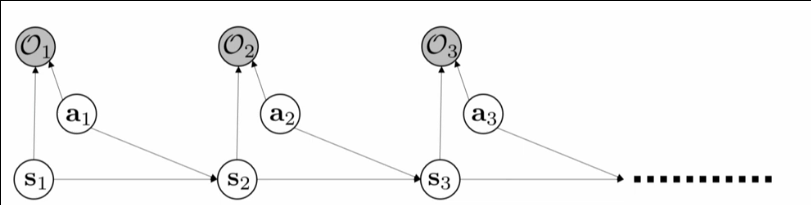
\includegraphics[width=0.8\linewidth]{figures/2020-07-06-130523_811x205_scrot.png}
\end{figure}

Como se está maximizando con respecto a $\psi$, el término de la dinámica $p(\tau)$ se puede
eliminar de \ref{eq:modelo_inv_tr}. Por lo que \ref{eq:ml_inv} se puede expresar como:
\begin{align}
    \label{eq:inv_ml_pre}
\operatorname { max } _ { \psi } \frac { 1 } { N } \sum _ { i = 1 } ^ { N } r _ { \psi } ( \tau _ { i } ) - \operatorname { log } Z
\end{align}
Donde $\log Z$ es un término que hace que todo sume a 1, ya que las probabilidades con
respecto a algo tienen que sumar hasta 1 (en este caso es respecto a $\tau$). Lo que
significa que $Z$ es la integral de todas las posibles trayectorias $\tau$ de $r_\psi(\tau)$.
$\log Z$ es la función de partición (\textit{partition function}). Esto es difícil de calcular
porque hay muchas trayectorias posibles (tiempo exponencial en sumarlas todas).

\subsection{La función de partición de RL inverso}%
\label{sub:la_función_de_partición_de_rl_inverso}

$Z$ se define como:
\begin{align}
Z = \int p ( \tau ) \operatorname { exp } ( r _ { \psi } ( \tau ) ) d \tau
\end{align}
La función de partición es necesaria ya que con maximizar la recompensa no basta, hay que
maximizarla para que tenga valores más altos que las recompensas de otras trayectorias. Usando
esta definición en \ref{eq:inv_ml_pre} y derivando se obtiene:
\begin{align}
\nabla _ { \psi } L = \frac { 1 } { N } \sum _ { i = 1 } ^ { N } \nabla _ { \psi } r _ { \psi } ( \tau _ { i } ) - \frac { 1 } { Z } \int p ( \tau ) \operatorname { exp } ( r _ { \psi } ( \tau ) ) \nabla _ { \psi } r _ { \psi } ( \tau ) d \tau
\end{align}
Sabiendo que:
\begin{align}
    p(\tau|O_{1:T},\psi)= \frac{1}{Z} \int p(\tau)\exp(r_\psi(\tau))
\end{align}
Se puede escribir lo anterior en forma de esperanza:
\begin{align}
    \label{eq:inv_grad}
\nabla _ { \psi } L = E _ { \tau \sim \pi ^ { \star } ( \tau ) } [ \nabla _ { \psi } r _ { \psi } ( \tau _ { i } ) ] - E _ { \tau \sim p ( \tau | O _ { 1 : T } , \psi ) } [ \nabla _ { \psi } r _ { \psi } ( \tau ) ]
\end{align}
Se puede ver que en esta expresión se toma como positivas las recompensas obtenidas de $\pi^*$
y se restan las recompensas obtenidas con  $\pi_\psi$. El gradiente será 0 cuando las
distribuciones sean iguales.

El primer término se estima usando muestras. El segundo término es el complicado de estimar
y el resto del tema tratará de varias técnicas para obtenerlo.

\section{Estimar la esperanza}%
\label{sec:estimar_la_esperanza}

Se recuerda que:
\begin{align}
E _ { \tau \sim p ( \tau | O _ { 1 : T } , \psi ) } [ \nabla _ { \psi } r _ { \psi } ( \tau ) ] =
E _ { \tau \sim p ( \tau | O _ { 1 : T } , \psi ) } \left[ \nabla _ { \psi } \sum _ { t = 1 } ^ {
    T } r _ { \psi } ( s _ { t } , a _ { t } ) \right]
\end{align}
Si se saca la suma fuera de la esperanza, se puede expresar con respecto al estado marginal
$(s_t,a_t)$ :
\begin{align}
E _ { \tau \sim p ( \tau | O _ { 1 : T } , \psi ) } \left[ \nabla _ { \psi } \sum _ { t = 1 } ^ {
    T } r _ { \psi } ( s _ { t } , a _ { t } ) \right]
= \sum _ { t = 1 } ^ { T } E _ { ( s _ { t } , a _ { t } ) \sim p ( s _ { t } , a _ { t } | O _ { 1 : T } , \psi ) } [ \nabla _ { \psi } r _ { \psi } ( s _ { t } , a _ { t } ) ]
\end{align}

Se usa la regla de la cadena para:
\begin{align}
( s _ { t } , a _ { t } ) \sim p ( s _ { t } , a _ { t } | O _ { 1 : T } , \psi )=
p ( a _ { t } | s _ { t } , O _ { 1 : T } , \psi ) p ( s _ { t } | O _ { 1 : T } , \psi )
\end{align}
Estos términos se han visto antes en el tema anterior. El primero es la política óptima
blanda (\textit{soft-optimal policy}), la cual con los mensajes hacia atrás se pueden calcular
esas probabilidades. El segundo término también se vio en el tema pasado al final de la tercera
pregunta.
\begin{align}
    p(a_t|s_t,O_{1:T},\psi)= \frac{\beta(s_t,a_t)}{\beta(s_t)} \\
    \propto \alpha(s_t)\beta(s_t)
\end{align}
Por lo que:
\begin{align}
p ( a _ { t } | s _ { t } , O _ { 1 : T } , \psi ) p ( s _ { t } | O _ { 1 : T } , \psi ) \propto \beta ( s _ { t } , a _ { t } ) \alpha ( s _ { t } )
\end{align}

Todo esto se está haciendo haciendo muchas asunciones. La más importante de ellas es que se
pueden enumerar todos los estados y acciones, calcular los mensajes $\alpha$ y $\beta$,
multiplicarlos entre ellos, y lo peor, normalizarlos, para que sea igual a y no proporcional.
Todo esto requiere que el espacio de acciones y estados sea lo suficientemente
pequeño como para hacer esto. Pero esta asunción ni se aproxima a las complicaciones de
calcular todas las trayectorias posibles, ya que es exponencial con respecto al tamaño del
espacio de estados, mientras que esto es lineal en el espacio de estados.

Se define $\mu_t$ :
\begin{align}
\mu _ { t } ( s _ { t } , a _ { t } ) \propto \beta ( s _ { t } , a _ { t } ) \alpha ( s _ { t } )
\end{align}
Por lo que:
\begin{align}
E _ { \tau \sim p ( \tau | O _ { 1 : T } , \psi ) } [ \nabla _ { \psi } r _ { \psi } ( \tau ) ]
&=
\sum _ { t = 1 } ^ { T } \int \int \mu _ { t } ( s _ { t } , a _ { t } ) \nabla _ { \psi } r _ {
\psi } ( s _ { t } , a _ { t } ) d s _ { t } d a _ { t }\\
&=\sum_{t=1}^T \overrightarrow{\mu}_t^T \nabla_\psi \overrightarrow{r}_\psi
\end{align}

Con esto, ya se tiene un algoritmo para hacer aprendizaje por refuerzo inverso:

\begin{algorithm}
    \caption{Máximum Entropy Inverse Reinforcement Learning}
    \Repeat{mientras se siga entrenando}{
        Dado $\psi$, calcular los mensajes hacia atrás $\beta(s_t,a_t)$ \\
        Dado $\psi$, calcular los mensajes hacia adelante $\alpha(s_t)$ \\
        Calcular $\mu_t(s_t,a_t)\propto\beta(s_t,a_t)\alpha(s_t)$ \\
        Evaluar: $ \nabla _ { \psi } L = \frac { 1 } { N } \sum _ { i = 1 } ^ { N } \sum _ { t =
        1 } ^ { T } \nabla _ { \psi } r _ { \psi } ( s _ { i , t } , a _ { i , t } ) - \sum _ { t
    = 1 } ^ { T } \int \int \mu _ { t } ( s _ { t } , a _ { t } ) \nabla _ { \psi } r _ { \psi }
    ( s _ { t } , a _ { t } ) d s _ { t } d a _ { t } $\\
        $\psi\gets\psi+\nu\nabla_\psi L$
    }
\end{algorithm}

Para espacios de estados pequeños y discretos esto funciona bastante bien.

Este método se llama \textit{Maximum Entropy} ya que se puede demostrar que en el caso en el que
la función de recompensa fuera lineal, este algoritmo da la solución que maximiza la entropía
de la política resultante de modo que la esperanza de las características de esta política es
igual a la esperanza de las características de la política del experto.
\begin{align}
\operatorname { max } _ { \psi } H ( \pi ^ { r _ { \psi } } ) \operatorname { de modo que } E _ { \pi ^ { r _ { \psi } } } [ f ] = E _ { \pi ^ { \star } } [ f ]
\end{align}

Esto tiene sentido ya que se está haciendo que a parte de correlacionar las características de
la función de recompensa, no se está asumiendo nada más del comportamiento.

Este algoritmo requiere:
\begin{itemize}
    \item Resolver la política óptima blanda en el bucle interno. Se calculan los
        mensajes. Básicamente se está resolviendo el problema de RL por cada paso del descenso
        por gradiente.
    \item Enumerar todas las tuplas acción-estado para obtener la frecuencia de visita y el
        gradiente.
\end{itemize}

Para poder aplicar esto en problemas prácticos, se tienen que relajar las asunciones:
\begin{itemize}
    \item Espacios de acciones y estados grandes y continuos.
    \item Tratar con estados obtenidos solamente de muestras.
    \item Tratar con dinámicas desconocidas.
\end{itemize}

\subsection{Con dinámica desconocida y espacio de acciones/estados grandes}%
\label{sub:con_dinámica_desconocida_y_espacio_de_acciones_estados_grandes}

Se asume que no se conoce la dinámica pero que se pueden sacar muestras como con RL.

Se recuerda que el gradiente viene dado por \ref{eq:inv_grad}, donde la primera parte se
calcula fácilmente pero la segunda no.

Se podría pensar en un algoritmo bueno pero impráctico que sería aprender
$p(a_t|s_t,O_{1:T},\psi)$ usando cualquier algoritmo \textit{Maximum Entropy RL algorithm}
(\textit{soft Q-Learning}, el algoritmo Policy Gradient con el término de la entropía, \ldots).
El problema es que esos se tienen que ejecutar hasta la convergencia para cada paso tomado en
$\psi$, aunque no requieren conocer las dinámicas ni enumerar los estados.

\begin{align}
\nabla _ { \psi } L \approx \frac { 1 } { N } \sum _ { i = 1 } ^ { N } \nabla _ { \psi } r _ { \psi } ( \tau _ { i } ) - \frac { 1 } { M } \sum _ { j = 1 } ^ { M } \nabla _ { \psi } r _ { \psi } ( \tau _ { j } )
\end{align}

Se pretenden realizar actualizaciones de $\psi$ que sean más eficientes con respecto a las
muestras. Para ello, en vez de aprender $p(a_t|s_t,O_{1:T},\psi)$ se va simplemente a
mejorar ligeramente usando un algoritmo de máxima entropía. Una forma de mejorarla
ligeramente por ejemplo es hacer un paso de policy gradient (esto funciona). Esto no nos va a dar
las muestras de $p(\tau|O_{1:T},\psi)$, pero nos dará las muestras de otra distribución en la
que a medida que vayamos tomando más pasos en el gradiente las muestras se irán pareciendo más
y más.

Para convertir muestras de una distribución a otra se puede usar Importance Sampling:

\begin{align}
    \nabla _ { \psi } L &\approx \frac { 1 } { N } \sum _ { i = 1 } ^ { N } \nabla _ { \psi } r _ {
\psi } ( \tau _ { i } ) - \frac { 1 } { \sum _ { j } w _ { j } } \sum _ { j = 1 } ^ { M } w _ { j
} \nabla _ { \psi } r _ { \psi } ( \tau _ { j } )\\
w _ { j } &= \frac { p ( \tau ) \operatorname { exp } ( r _ { \psi } ( \tau _ { j } ) ) } { \pi ( \tau _ { j } ) }
\end{align}
Expandiendo la expresión para los pesos:
\begin{align}
w _ { j } = \frac { p ( \tau ) \operatorname { exp } ( r _ { \psi } ( \tau _ { j } ) ) } { \pi ( \tau _ { j } ) }
=
\frac { p ( s _ { 1 } ) \prod _ { t } p ( s _ { t + 1 } | s _ { t } , a _ { t } ) \operatorname { exp } ( r _ { \psi } ( s _ { t } , a _ { t } ) ) } { p ( s _ { 1 } ) \prod _ { t } p ( s _ { t + 1 } | s _ { t } , a _ { t } ) \pi ( a _ { t } | s _ { t } ) }
=
\frac{\exp(\sum_t r_\psi(s_t,a_t))}{\prod_t\pi(a_t|s_t)} 
\end{align}
El denominador resultante es difícil de trabajarlo, pero es un paso en la buena dirección.

En general, Importance Sampling no es una buena idea usarlo si se trata de dos distribuciones
muy distantes. Aquí las distribuciones pueden ser distantes al principio pero por cada
actualización de $r_\psi$ las trayectorias se irán pareciendo más y más, por lo que no es
descabellado usarlo.

El primer algoritmo que usó esta estructura fue \textit{ Guided Cost Learning Algorithm, Finn et
al. ICML 2016. }
\begin{figure}[H]
	\centering
	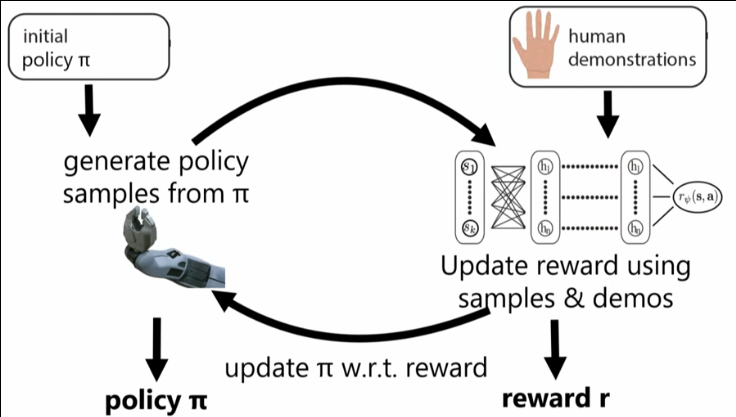
\includegraphics[width=0.5\linewidth]{figures/2020-07-06-161322_736x417_scrot.png}
\end{figure}

Este algoritmo puede ser interpretado como un ascenso por gradiente con respecto a $\psi$.
Pero también se puede interpretar que $r_\psi$ se actualiza, aumenta la recompensa del
experto y disminuye la del agente, y cuando se actualiza la política intenta que su recompensa
sea máxima.

\begin{figure}[H]
	\centering
	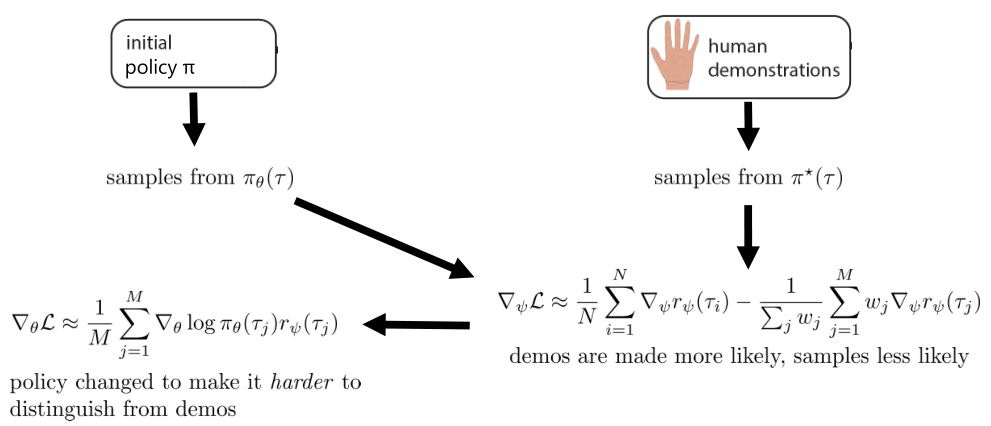
\includegraphics[width=0.8\linewidth]{figures/2020-07-06-161727_991x426_scrot.png}
\end{figure}

El objetivo final es hacer que la política $\pi_\theta$ sea indistinguible de la política del
experto $\pi^*$. El único equilibrio es resolver el problema del aprendizaje por refuerzo
inverso.

Esto se parece mucho a una GAN. La política tiene el rol del generador, y la función de
recompensa el discriminador.

En el caso de aprendizaje por refuerzo inverso, el mejor discriminador es:
\begin{align}
D ^ { \star } ( x ) = \frac { p ^ { \star } ( x ) } { p _ { \theta } ( x ) + p ^ { \star } ( x ) }
\end{align}
como la política óptima se acerca a $\pi_\theta(\tau)\propto
p_(\tau)\exp(r_\psi(\tau))$, se elige la siguiente parametrización para el discriminador:
\begin{align}
D _ { \psi } ( \tau ) = \frac { p ( \tau ) \frac { 1 } { Z } \operatorname { exp } ( r ( \tau ) )
} { p _ { \theta } ( \tau ) + p ( \tau ) \frac { 1 } { Z } \operatorname { exp } ( r ( \tau ) ) }
=
\frac { p ( \tau ) \frac { 1 } { Z } \operatorname { exp } ( r ( \tau ) ) } { p ( \tau ) \prod _ { t } \pi _ { \theta } ( a _ { t } | s _ { t } ) + p ( \tau ) \frac { 1 } { Z } \operatorname { exp } ( r ( \tau ) ) }
=
\frac { \frac { 1 } { Z } \operatorname { exp } ( r ( \tau ) ) } { \prod _ { t } \pi _ { \theta } ( a _ { t } | s _ { t } ) + \frac { 1 } { Z } \operatorname { exp } ( r ( \tau ) ) }
\end{align}
Esta expresión no se puede escribir para GAN en otros ámbitos porque aquí conocemos
$\pi_\theta$.

Ahora se optimiza el discriminador con respecto a $\psi$. Si se escribe el objetivo del
discriminador de antes y le metemos esta definición de discriminador se obtiene:
\begin{align}
\psi \leftarrow \operatorname { arg } \operatorname { max } _ { \psi } E _ { \tau \sim p ^ { \star } } [ \operatorname { log } D _ { \psi } ( \tau ) ] + E _ { \tau \sim \pi _ { \theta } } [ \operatorname { log } ( 1 - D _ { \psi } ( \tau ) ) ]
\end{align}
Se obtiene una expresión que coincide con el gradiente de RL inverso.

Sorprendentemente, también se puede optimizar $Z$ con respecto a $\psi$ en el objetivo y se
obtiene el valor correcto de $Z$.

La explicación de esto está en la publicación: \textit{ Finn\", Christiano\" et al. \"A Connection Between Generative Adversarial Networks, Inverse Reinforcement Learning, and Energy-Based Models.\" }

\begin{figure}[H]
	\centering
	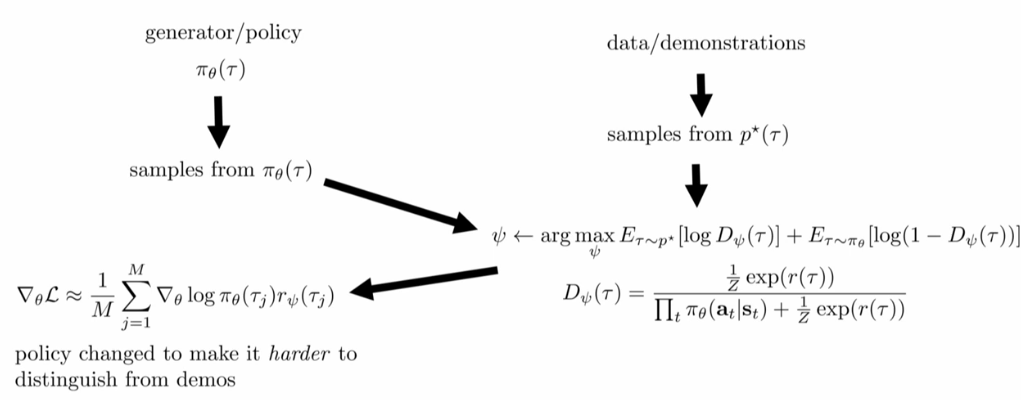
\includegraphics[width=0.8\linewidth]{figures/2020-07-06-164555_1021x400_scrot.png}
	\caption{Algoritmo de IRL}
\end{figure}

Si solo nos preocupa la política obtenida y no la explicación de las acciones de los
agentes, se puede usar un método más parecido a una GAN literalmente:
\begin{figure}[H]
	\centering
	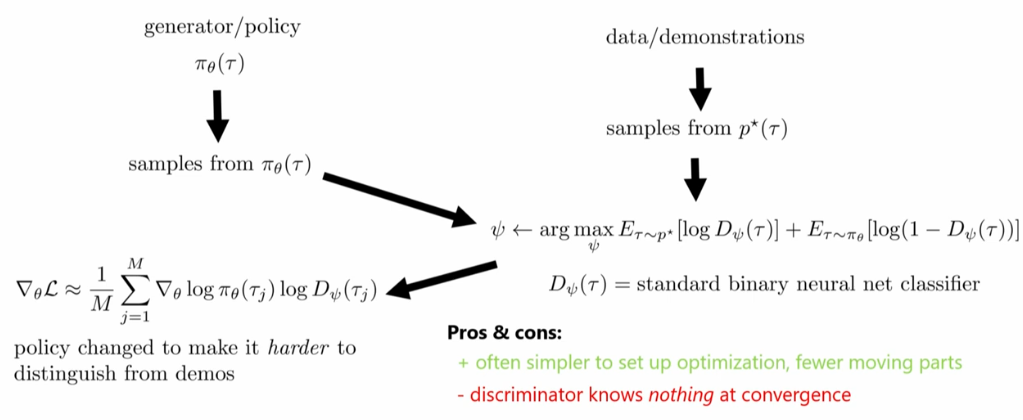
\includegraphics[width=0.8\linewidth]{figures/2020-07-06-165353_1023x420_scrot.png}
\end{figure}
En resumen, en vez de minimizar y maximizar, lo que se hace es tener un discriminador
binario. $ D(\tau)$ es la probabilidad de que $\tau$ sea una demostración y no una trayectoria
generada por el agente. Se usa $D(\tau)$ como \"recompensa\".

